\documentclass[8pt, a4paper]{article}
\usepackage[utf8]{inputenc}
\usepackage{graphicx}
\usepackage{hologo}

\graphicspath{ {images/} }

\title{lorecast162's first doc}
\author{lorecast162}


\begin{document}
\maketitle
This is my first ever piece of text written using LaTeX.
Damn this shit \textit{hard} man.

This is a picture of a cat.
\begin{figure}[h]
  \centering
  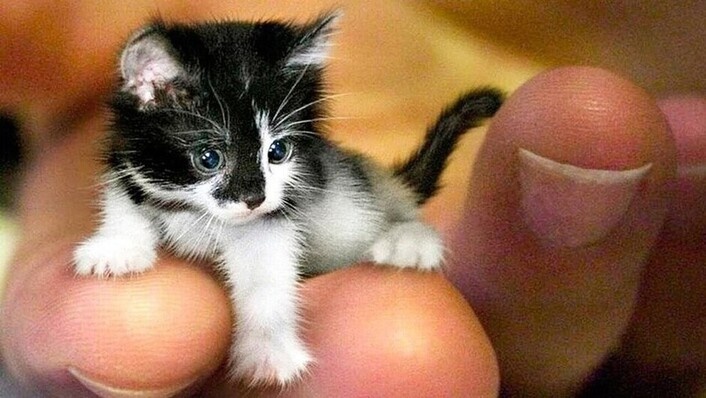
\includegraphics[width=0.5\textwidth]{cat}
  \caption{\emph{Look at this cute little kitten, delightful.}}
  \label{fig:catto}
\end{figure}

\[
\int x^5 * x\lambda^y
\]

\hologo{LaTeX}

I could remain here all day describing just
how calming the cat in figure \ref{fig:catto}
in page \pageref{fig:catto} is.



\end{document}
